\documentclass[../Main.tex]{subfiles}
\begin{document}

\section{Design an Enjoyable Game}

        How to create an enjoyable game is an important part of every game development process. This chapter presents a literature study of the subject based on work conducted by \citeauthor{malone_what_1980} in \citeyear{malone_what_1980}, “What makes things fun to learn?”, and \citeauthor{sweetser_gameflow_2005}’s “GameFlow: a model for evaluating player enjoyment in games”. \citeauthor{malone_what_1980}’s research outlines challenge, fantasy, and curiosity as three main elements that increase motivation. The GameFlow article presents a model for evaluating enjoyment in games. 
        
        
        \citep{malone_what_1980-1}.
        \citep{malone_what_1980}.
    \subsection{What makes things fun to learn?}
        \subsubsection{Challenge}
        
        \subsubsection{Fantasy}
        
        \begin{figure}[H]
            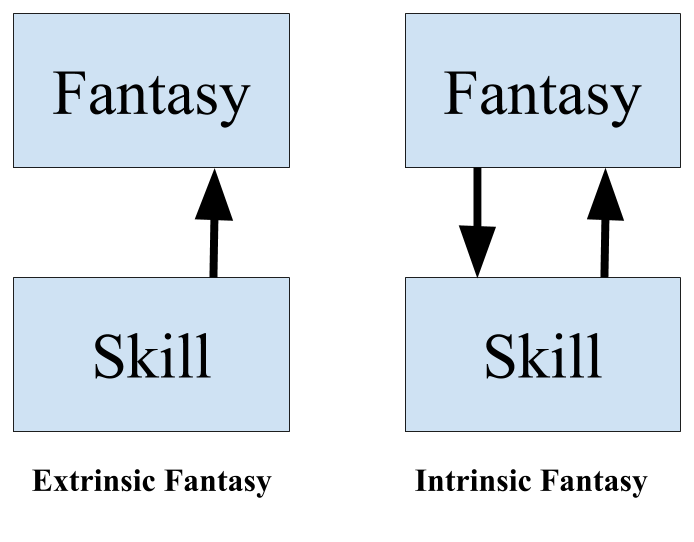
\includegraphics[width=1\textwidth]{Images/SkillFantasy.png}
            \caption{Logical dependencies in extrinsic and intrinsic fantasies}
            \label{fig:skill_fantasy}
        \end{figure}
        \citep{lazzaro_four_2008}
        \subsubsection{Curiosity}
        
   \subsection{Gameflow}
        \subsubsection{Concentration}
        \subsubsection{Challenge}
        \subsubsection{Skills}
        \subsubsection{Control}
        \subsubsection{Clear goals}
        \subsubsection{Feedback}
        \subsubsection{Immersion}
        \subsubsection{Social interaction}


\biblio % Needed for referencing to working when compiling individual subfiles - Do not remove
\end{document}